\subsection{The check with a complete reference}\label{s:works}

\begin{figure*}[t]
  \centering
  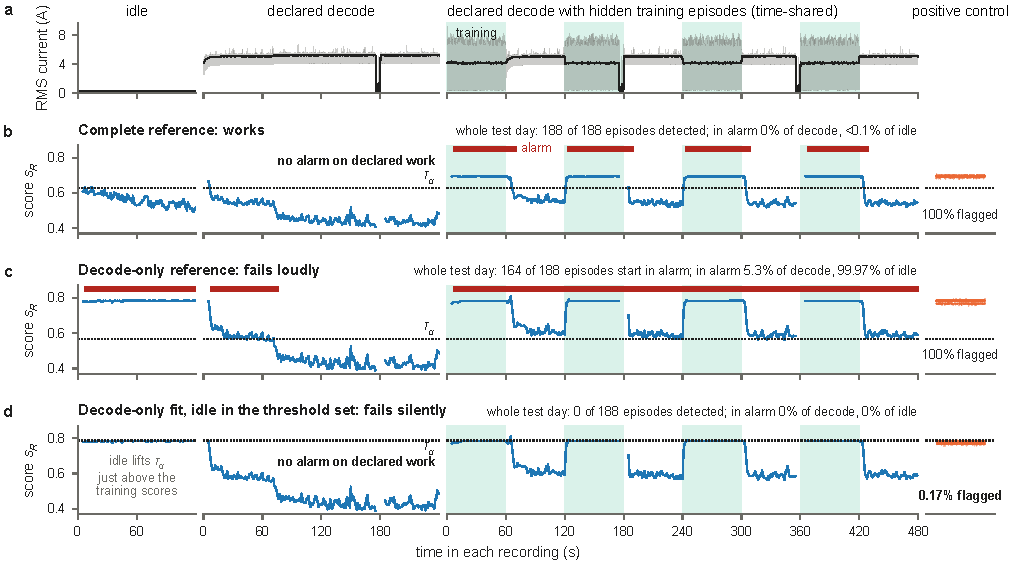
\includegraphics[width=\linewidth]{f8_monitors.pdf}
  \caption{Three configurations of the signature check on the same test-day recordings.
    (a) RMS current in three separate recordings: idle, declared decode, and decode with
    time-shared training episodes (shaded). Line: mean of $e(t)$ per \FeightBin~s; band:
    its 5--95\% range. The dips are unscored seconds. (b)--(d) The score $s_R$, the
    threshold $\tau_\alpha$ (dotted) and the alarm (red bar). (b) The fit holds decode,
    prefill and idle; the threshold set holds decode and idle. (c) Both hold decode only.
    (d) The fit holds decode only; the threshold set holds decode and idle. Right column:
    $s_R$ of honest-training windows from the development data, a positive control.}
  \label{f:f8}
\end{figure*}

The signature check needs no examples of hidden training. With the complete reference, whose fit
holds decode, prefill and idle, $s_R$ at $\tau_\alpha = \TauRone$ detects
$\Ztwo\%$ of co-location windows (development data, one run per training share), and at
least \RoneMinGroup\% of every other evasion group, although it is fitted to
none of them. Its test false-positive rates are \FprRoneDecode\% on decode
and \FprRoneIdle\% on idle.

We also run $s_R$ over the test day as a monitor (\cref{s:monitor}; \cref{f:f8}b).
That day embeds \EpTotal{} time-shared training episodes of \EpMinDur{}~s to
\EpMaxDur{}~s inside declared inference. An episode is detected iff an alarm is active
at some time $t \in [t_{\mathrm{s}},\, t_{\mathrm{e}} + \Grace~\mathrm{s}]$, where its
first step starts at $t_{\mathrm{s}}$ and it ends at $t_{\mathrm{e}}$. An episode with
no alarm is missed, even if it is too short to hold a complete step. We leave out
\EpTruncated{} episodes that the recording cuts short. Both $s_R$ and the classifier, $s_C^{\mathrm{dev}}$,
detect all of the other \EpScored. For $s_R$ the median delay from
first step to alarm onset is $D = \EpDelayRone$~s, and even the shortest episodes
(\LminRone~s) have a within-run lower bound on detection above the target level
of \LminLevel. $s_R$ raises no alarm on test-day decode (\cref{t:t2}). These episodes
test time-sharing only; no co-located episode was recorded.

These results do not hinge on $\alpha$ or on the alarm rule. For $\alpha$ from 1\% to 10\%,
$s_R$ detects \RobCoMin\% of co-location windows and all \EpScored{} episodes, with
\RobOnDecAlpha{} false-alarm onsets on test-day decode and at most \RobOnIdleAlpha{} on idle. Under
persistence rules from 2-of-3 to 5-of-5 it still detects all \EpScored{} episodes, with at
most \RobOnDecPers{} onsets on decode and \RobOnIdlePers{} on idle.
